
\subsection{Supervised Learning}
\label{sec:supervised_learning}

Supervised learning can be generally thought of as function approximation where, given a set of inputs and expected outputs, a function from the input to the output is approximated by using a set of learning rules. The input and output of the approximate function depends on the input and output specified by the question posed by the data. Supervised learning can be broken down into two main branches: label classification and regression prediction. 

\subsubsection{Label classification}
\label{sec:label_classification}
The simplest form of label classification is often referred to as binary classification, in which the classifier (machine learning algorithm) has to discriminate between two classes. For example, a simple binary classification problem would be to discriminate between sets of points on a cartesian plane (Fig. \ref{fig:two_classes_example}).

\begin{figure}[!h]
  \centering
  \begin{subfigure}{.49\textwidth}
    \centering
    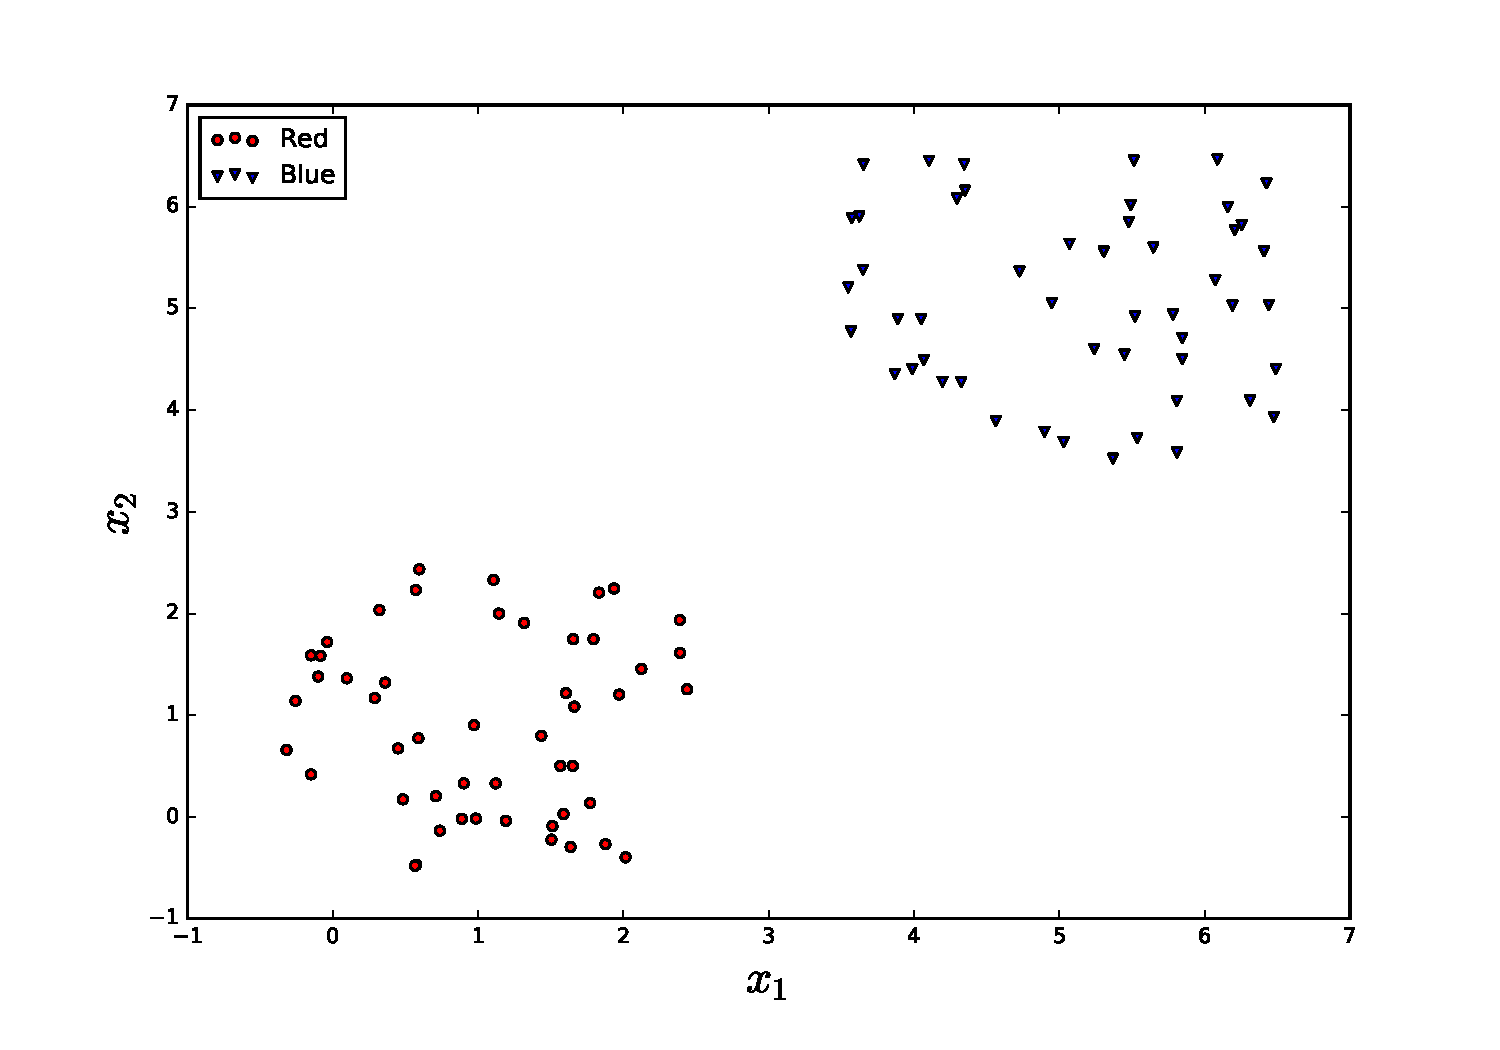
\includegraphics[width=\linewidth]{figures/twoClasses_separable.pdf}
  \end{subfigure} %
  \begin{subfigure}{0.49\textwidth}
    \centering
    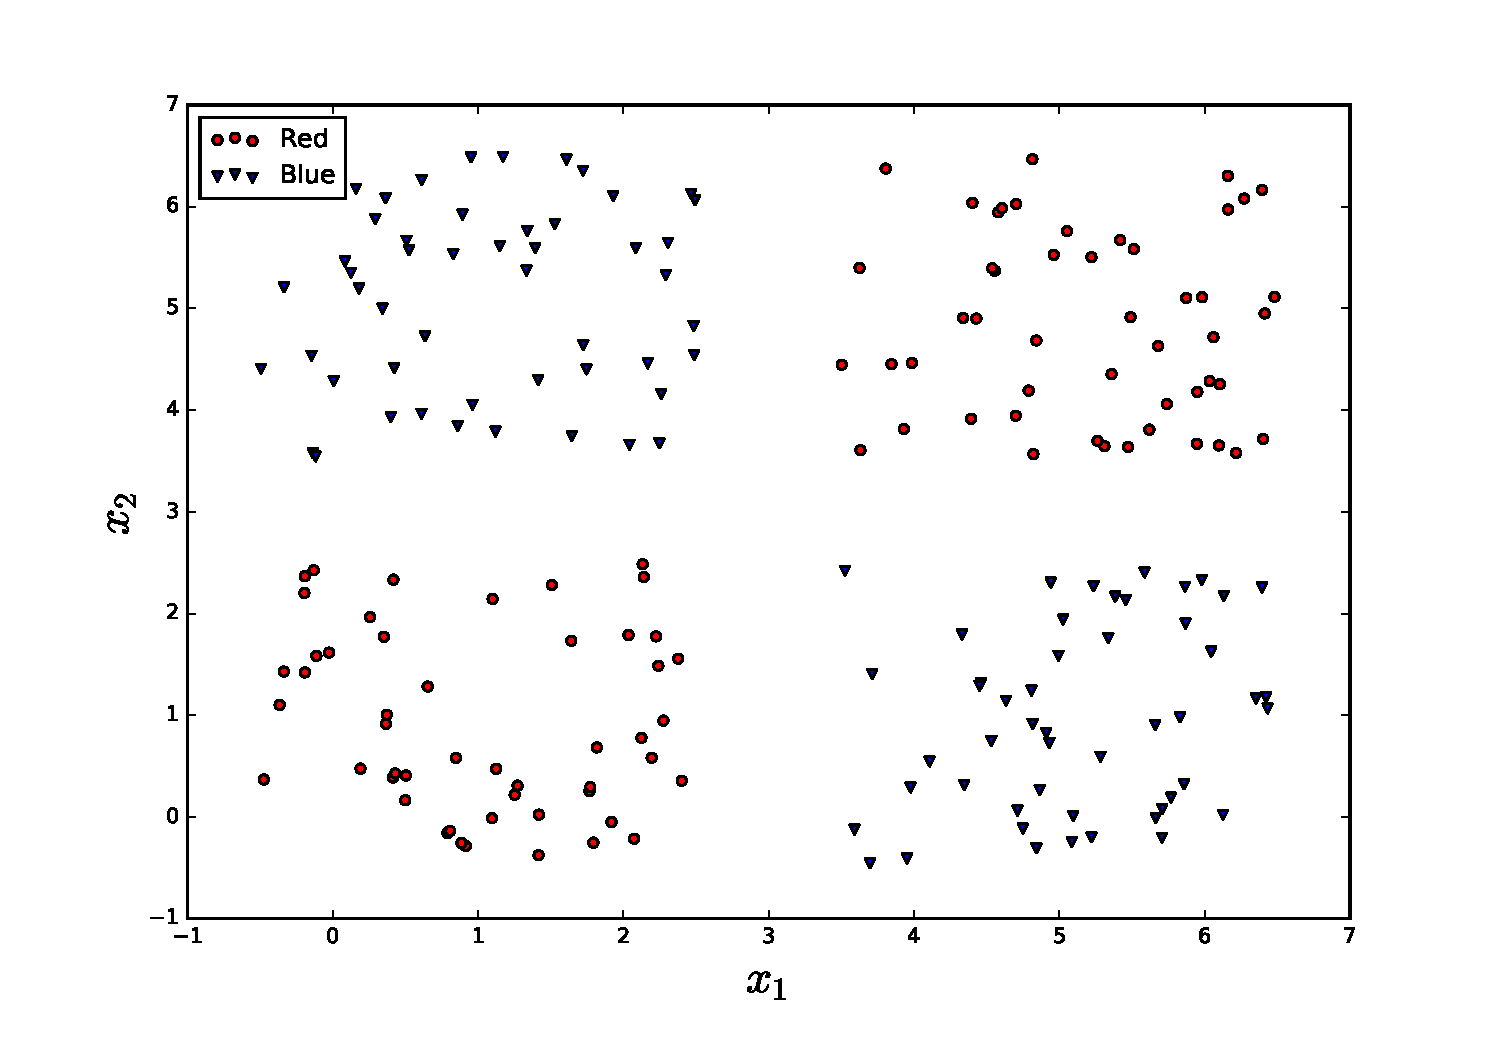
\includegraphics[width=\linewidth]{figures/twoClasses_non_separable.pdf}
  \end{subfigure}
  \caption{Two sets of data, one of which is linearly separable (Left) and the other is non linearly separable (Right). Linear separability means that a line can be found that can perfectly segregate the two classes into two sections. A diagonal, horizontal, or vertical line between the blue and red points can be drawn on the left that achieves that goal. However, on the right there is no one line that can be used to separate the data. This problem of finding a line of separation between two linearly seprable data sets can be solved by using a binary classifier, the earlierst example of which is the perceptron.}
  \label{fig:two_classes_example}
\end{figure}

 The perceptron was the first machine learning algorithm designed to solve binary classification in linearly separable conditions. Perceptrons were designed to mimick the McCollough-Pitts neuron model which relied on three main components: inputs, weights, and an activation function. In addition to these components, the perceptron had a learning rule that allowed it to learn when to and not to fire. Listing all the components of a perceptron:
\begin{itemize}
  \item \textbf{Inputs}: A dataset of $n$ dimensional points. Each input point $x$ consists of $n$ features such that each input point can be describes as $(x_1, x_2, \dots, x_n)$.
  \item \textbf{Weights}: $n$ weights described as $w_1, w_2, \dots, w_n$.
  \item \textbf{Activation}: a threshold $\theta$ on which the neuron decides to fire.
  \item \textbf{Learning Rule}: A rule by which the weights change, described below.
\end{itemize}

% After being trained, the perceptron would fire to indicat that it has seen one class of data points (+1) and would not fire to indicate that it has seen the other class of data points (-1). 

A perceptron can be trained by passing each data point from the the dataset to it. In our example (Fig. \ref{fig:two_classes_example}), each data point would have a two -dimensional input consisting of the $x_1$ and $x_2$ values. Since we are working with two dimensions, the perceptron would have two weights $w_1$ and $w_2$. Every 1time the perceptron encounters a data point it tries to make a prediction by calculating the weighted sum of the inputs $S$  as $\sum_{i=1}^n w_ix_i$. If $S \geq \theta$ then the neuron fires, meaning it predicts the category to be $+1$. If $S < \theta$, the neuron doesn't fire, predicting the category to be $-1$. Given this determination, the perceptron evaluates its predicted output with the actual output of the data point, then manipulating its weights, completing the learning process of the perceptron on that data point. 

The learning proccess for input $x$, given a true label $\gamma$ and a threshold $\theta$ is summarized by the following updates:
\begin{align}
  S &= \sum_{i=1}^n w_i*x_i > 0  \\
  \kappa &= \begin{cases} 
    +1 \textrm{ if $S$} > \theta \\
    -1 \textrm{ otherwise} 
  \end{cases} \\
  w_{new} &= w_{old} + (\kappa - \gamma)x.
\end{align}

As can be seen from above, the perceptron learns by changing its weights, as this causes the same input to give a different $S$ which in turn could give a different predicted value $\kappa$. Following this learning rule, it can be proven that the perceptron model converges in finite time to a set of weights result in a perfect classification for all data points in the dataset. A simple implementation of the perceptron was used to solve the sample datasets presented earlier (Fig \ref{fig:perceptron_solution}).

\begin{figure}[!h]
  \centering
  \begin{subfigure}{.49\textwidth}
    \centering
    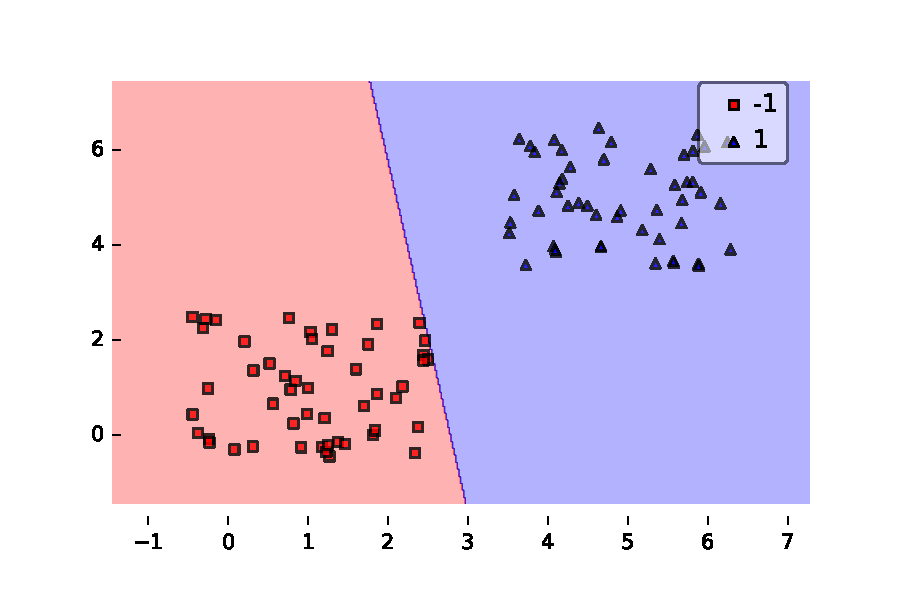
\includegraphics[width=\linewidth]{figures/perceptron_solvable.pdf}
  \end{subfigure} %
  \begin{subfigure}{0.49\textwidth}
    \centering
    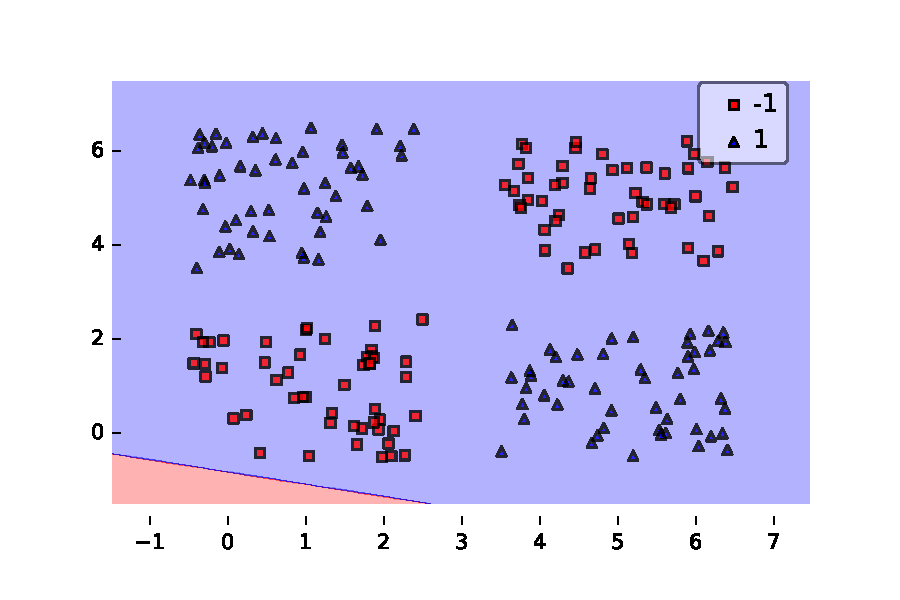
\includegraphics[width=\linewidth]{figures/perceptron_non_solvable.pdf}
  \end{subfigure}
  \caption{The perceptron model can be used to solve binary classification in linearly separable datasets as in the left image. After training, all points below the shown line of separation would be classified as -1, and all points above the line would be classified as +1. Seemingly, this behavior would correctly extrapolate to unseen datapoints from a similar distribution. In the case of non linearly separable datasets, the perceptron keeps adjusting its weights but never reaches a solution which correctly classifies all data inputs, meaning the model quits after a set limit of iterations through the dataset. This results in a having a line that clearely does not separate the two classes (Right).}
  \label{fig:perceptron_solution}
\end{figure}



  %TODO: Could talk about how to find if a datset is linearly separable. Could we use Perceptrons to do it?




In this subset of supervised learning, the input and output are both categorial data, as apposed to numbers in a range. The cononical example of categorial data for supervised learning is swimming pool opening based on weather conditions. In this example, there are several weather-related features such as \textit{Outlook, Temperature, Humidity,} and \textit{Windy}. The \textit{Outlook} feature could contain categories such as sunny, overcast, or rainy; the \textit{Temperature} feature could include categories such as hot or cold; the windy category could include false or true. All these features contain values from finite set of possiblities. 



Table \ref{table:categorial_examples_weather} shows possible data points of such a dataset. From this small sample, a general rule for playing like 

\begin{align*}
  	\textrm{If outlook}&=\textrm{sunny } \wedge \textrm{ humidity = high} \\
	\textrm{If outlook}&= \textrm{rainy} \wedge \textrm{windy = true}
\end{align*}

can be formulated. Atlhough this might be a good rule to follow, it might not generalize well to the rest of the dataset, and inspecting the entire dataset by eye becomes unfeasable beyong $~20$ datapoints. A common approach to solving this problem is called a Decision Tree. In this algorithm, the datapoints are iteratively separated by the feature that splits the data most evenly. For example,
NEED TO INCLUDE FORMULA FOR INFORMATION GAIN AND CATEGORY SEPARATION FOR DECISION TREES.
\begin{center}
 \label{table:categorial_examples_weather}
 \begin{tabular}{||c c c c c||} 
 \hline
 Outlook & Temperature & Humidity & Windy & Play \\ [0.5ex] 
 \hline\hline
 Sunny & Hot & High & false  & no\\ 
 \hline
 Sunny & Hot & High & true  & no\\ 
 \hline
 Overcast & Hot & High & false  & yes\\ 
 \hline
 Rainy & Mild & High & false  & yes\\ 
 \hline
 Rainy & Cool & Normal & false  & yes\\ [1ex] 
 \hline
\end{tabular}
\end{center}
%caption: A sample set of datapoints that could be present in the weather data set. All features are categorial, meaning the values of the features are from a finite, relatively small set of possibilities. The values can not be numerically represented in a forumula or compared, nor do they represent values on a range.


For example, if the input takes the form of images that contain a number and the output (labels of the images) is a number from 0 to 9, then the function would produce a mapping from a set of image properties to the set of numbers 0 to 9. Conversely, if the input is a set of numbers each representing a cost

\subsubsection{Regression Prediction}
\label{sec:regression_supervised_learning}
For cases when the desired output of a function is a number on a meaningful range, label classification is not possible. This is because a supervised label classification problem deals with \textit{choosing} the best label out of a given set, and not generating a label out of the given data. This is where regression prediction comes into play. For functions whose output is a continuous range of numbers, one can not possibly assign a label to each possible output. And even if each output is assignable, there is rarely a dataset big enough to cover possible mappings to each such label.

For example, given an input set of ${1,2,3,4,5,6,7}$ and an output set ${1,4,9,14,25,36,49}$, a good---and almost any---supervised learning algorithm would approximate the function $f(x^2)$. However, such a function would have rely on regression learning, and not label classification. To show this, let's delve into a thinking exercise. Say we make a training set for the function $f(x) = x^2$ consisting of input that is all the integers from one to one million and output that is the square of all these input numbers. If we are to use label classification, then we would train the algorithm to map each number to its square label. The first problem arrises on the first step of learning, especially in the Decision Tree technique. Because each input is looked at as a categorial input, an input of one (1) will be converted to a string. Sicne each data point has its own label, the information gain will be maximized and the entropy loss will be minimized when the input is split into one million branches on the first level of the tree. At that point, the function mapping is resolved by simply going through one level. However, this leads to the second problem, which arrises when feeding in new test data that the classifier was not trained on. Because the classifier only has access to labels that it trained on, any number other than an integer from one to million will have to map to an already known label from the squares of the integeres from one to one million. For example, an input of $1.76$ will map to either $1$ ($1^2=1$) or $4$ ($2^2 = 4$), meaning this encurs an accuracy cost. This cost might not be a big problem for the purposes of the algorithm, but the real problem arises when we try to predict the mapping of a number outside the range of our training dataset: numbers below 0 and those above one million. The nearest value for all numbers below 0 is 
$1$, so all the numbers below 0 will be mapped to the label of $0$, while all the numbers above one million will be mapped to the label of one million (Fig \ref{fig:decision_tree_regression_and_classification}).

\begin{figure}[!h]
  \centering
  \begin{subfigure}{.49\textwidth}
        \centering
        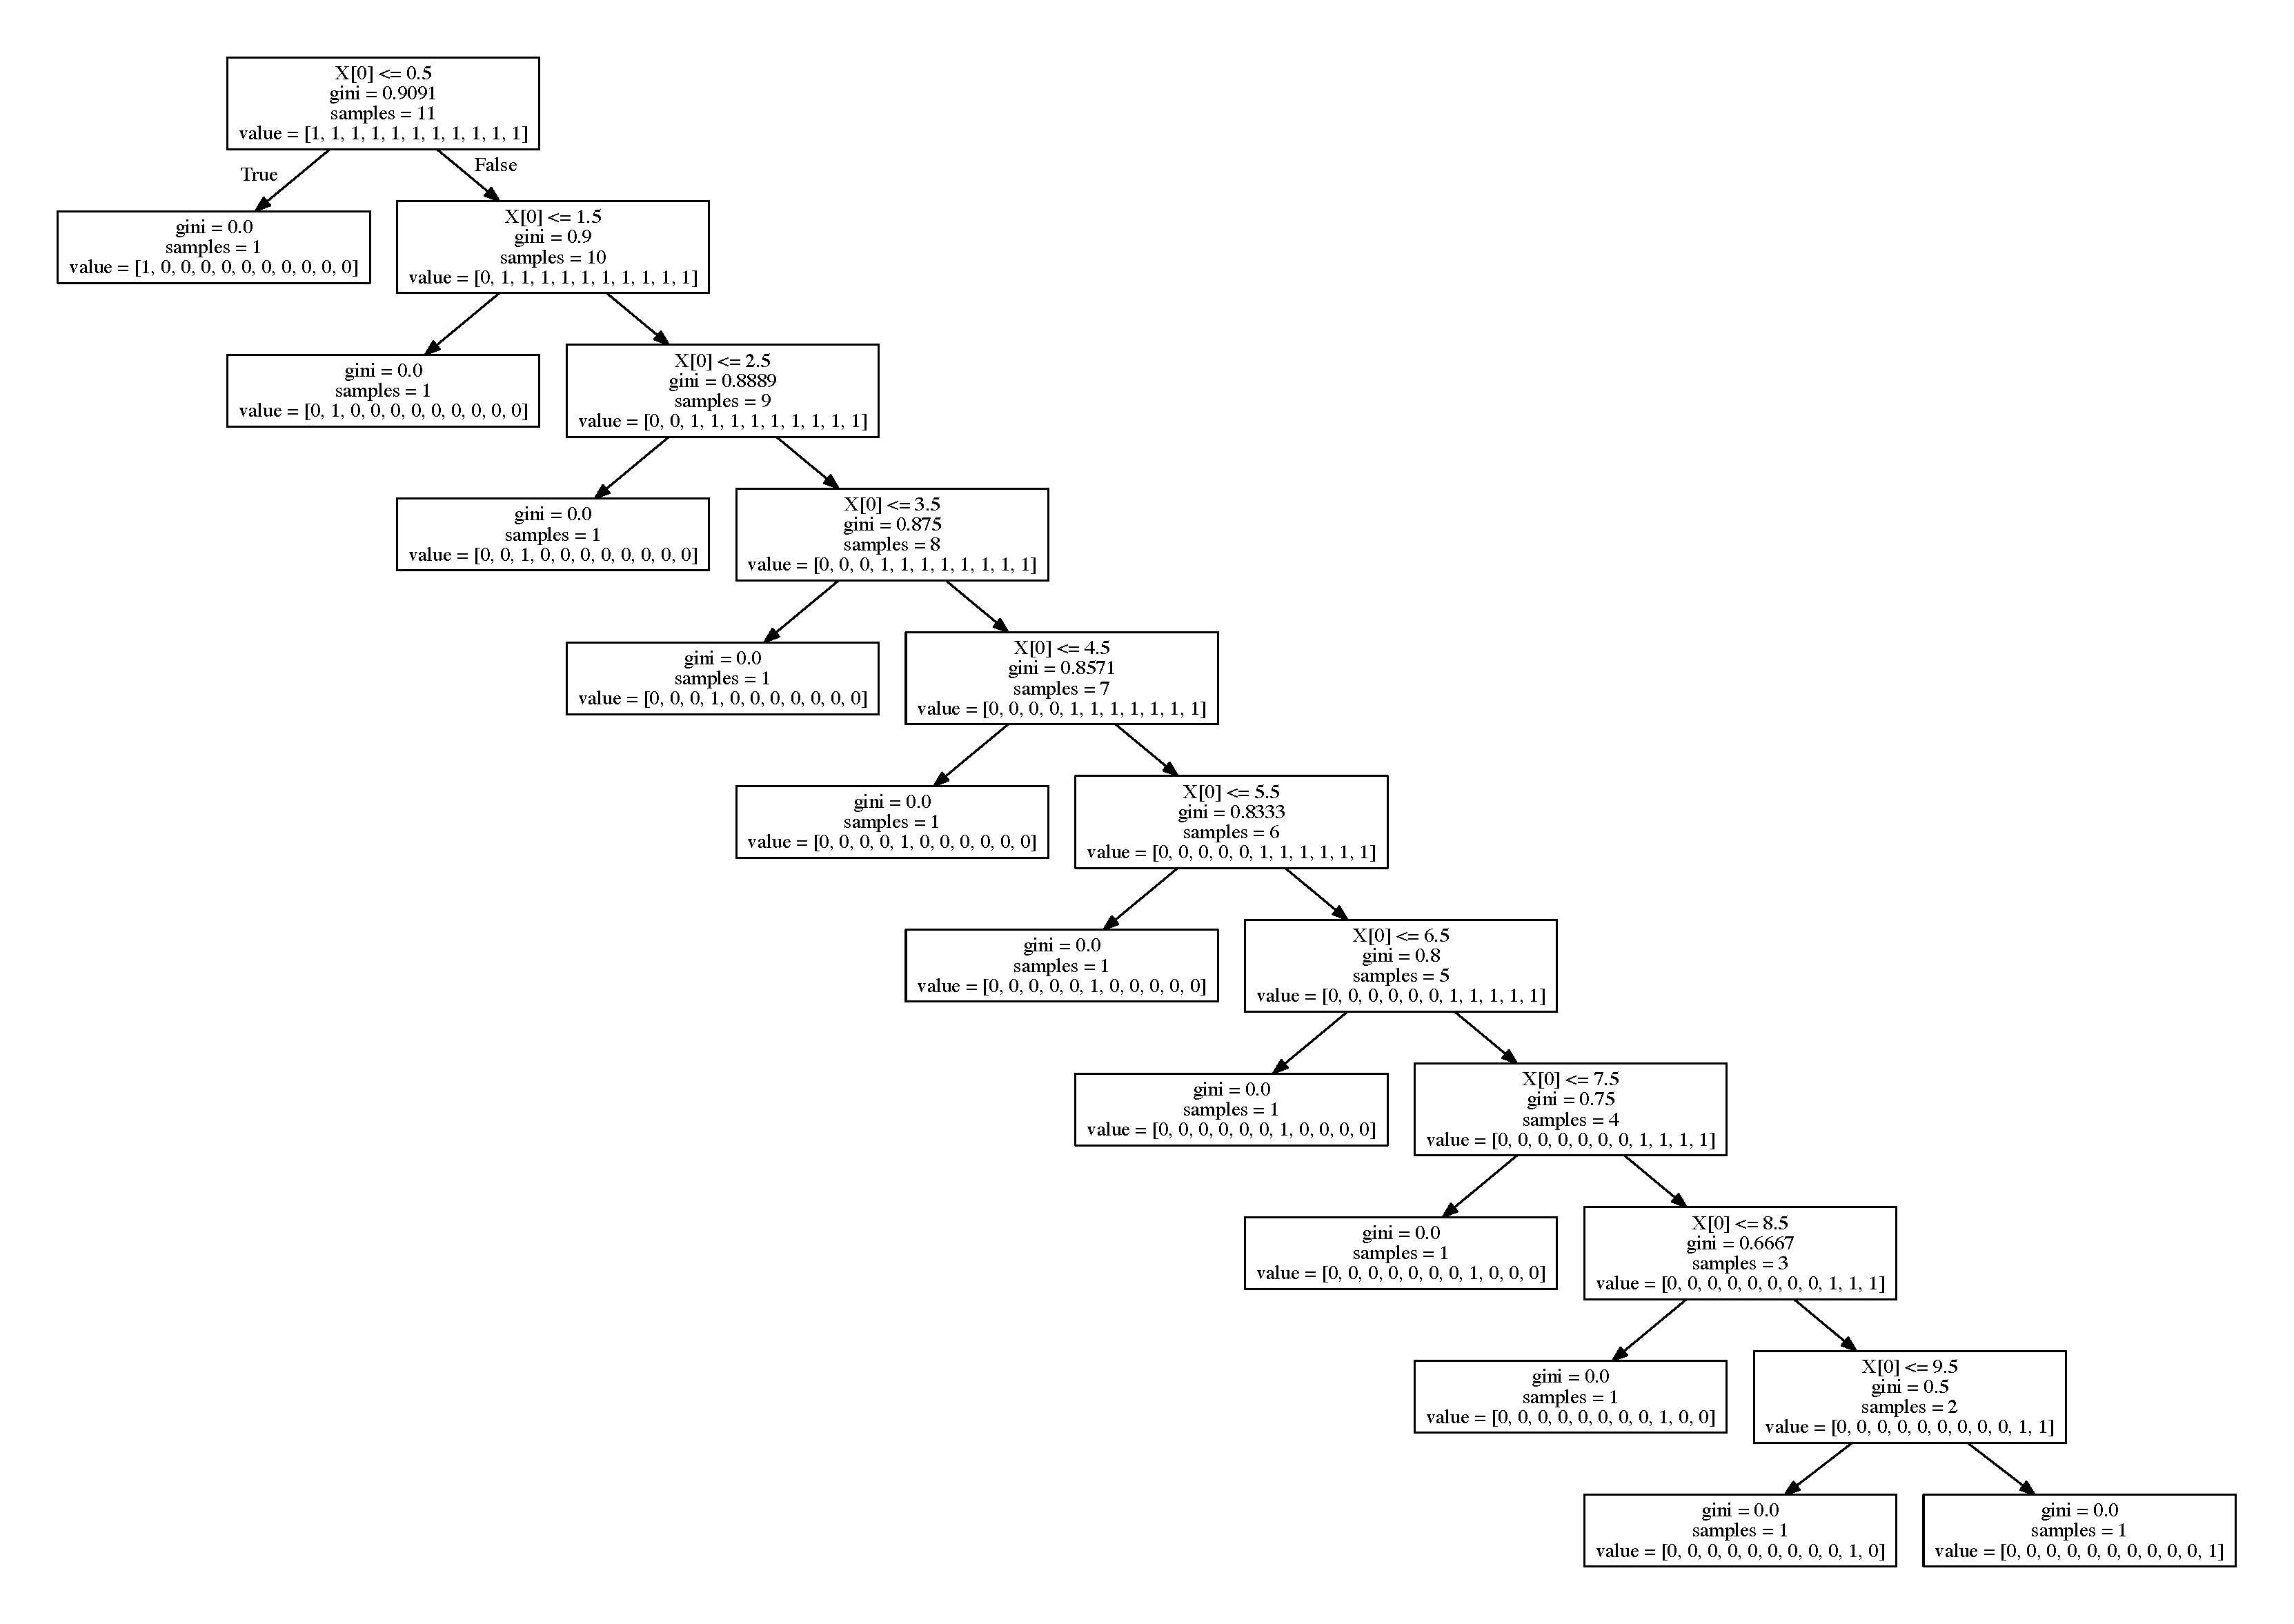
\includegraphics[width=\linewidth]{figures/clas_tree.pdf}
        \caption{Classification Decision Tree}
    \end{subfigure} %
    \begin{subfigure}{0.49\textwidth}
        \centering
        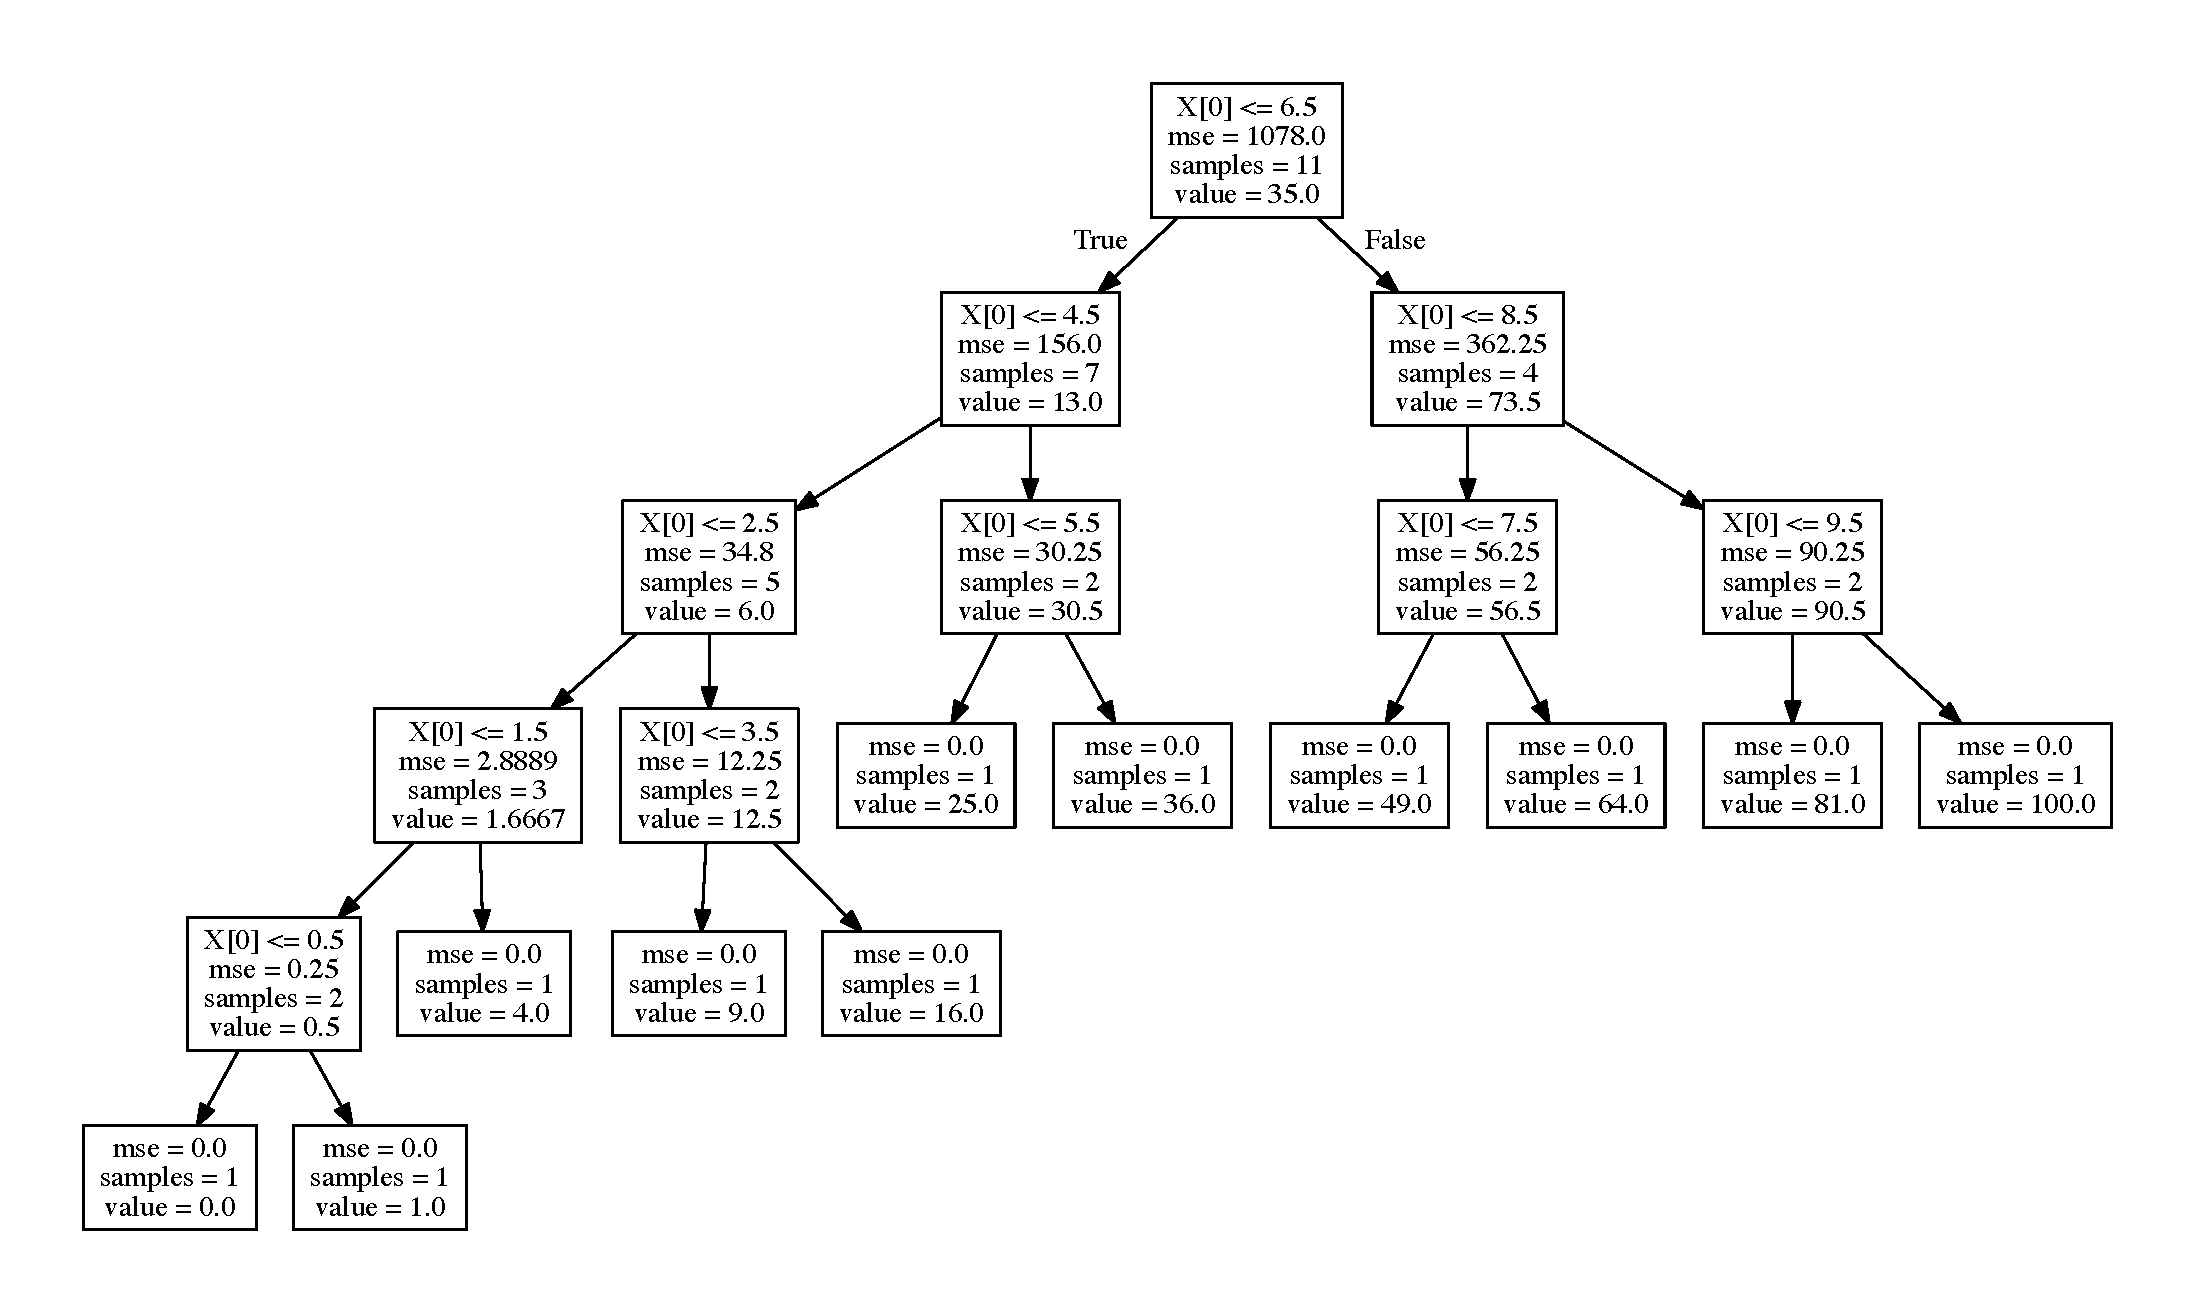
\includegraphics[width=\linewidth]{figures/reg_tree.pdf}
        \caption{Regression Decision Tree}
    \end{subfigure}
  \begin{subfigure}{.49\textwidth}
        \centering
        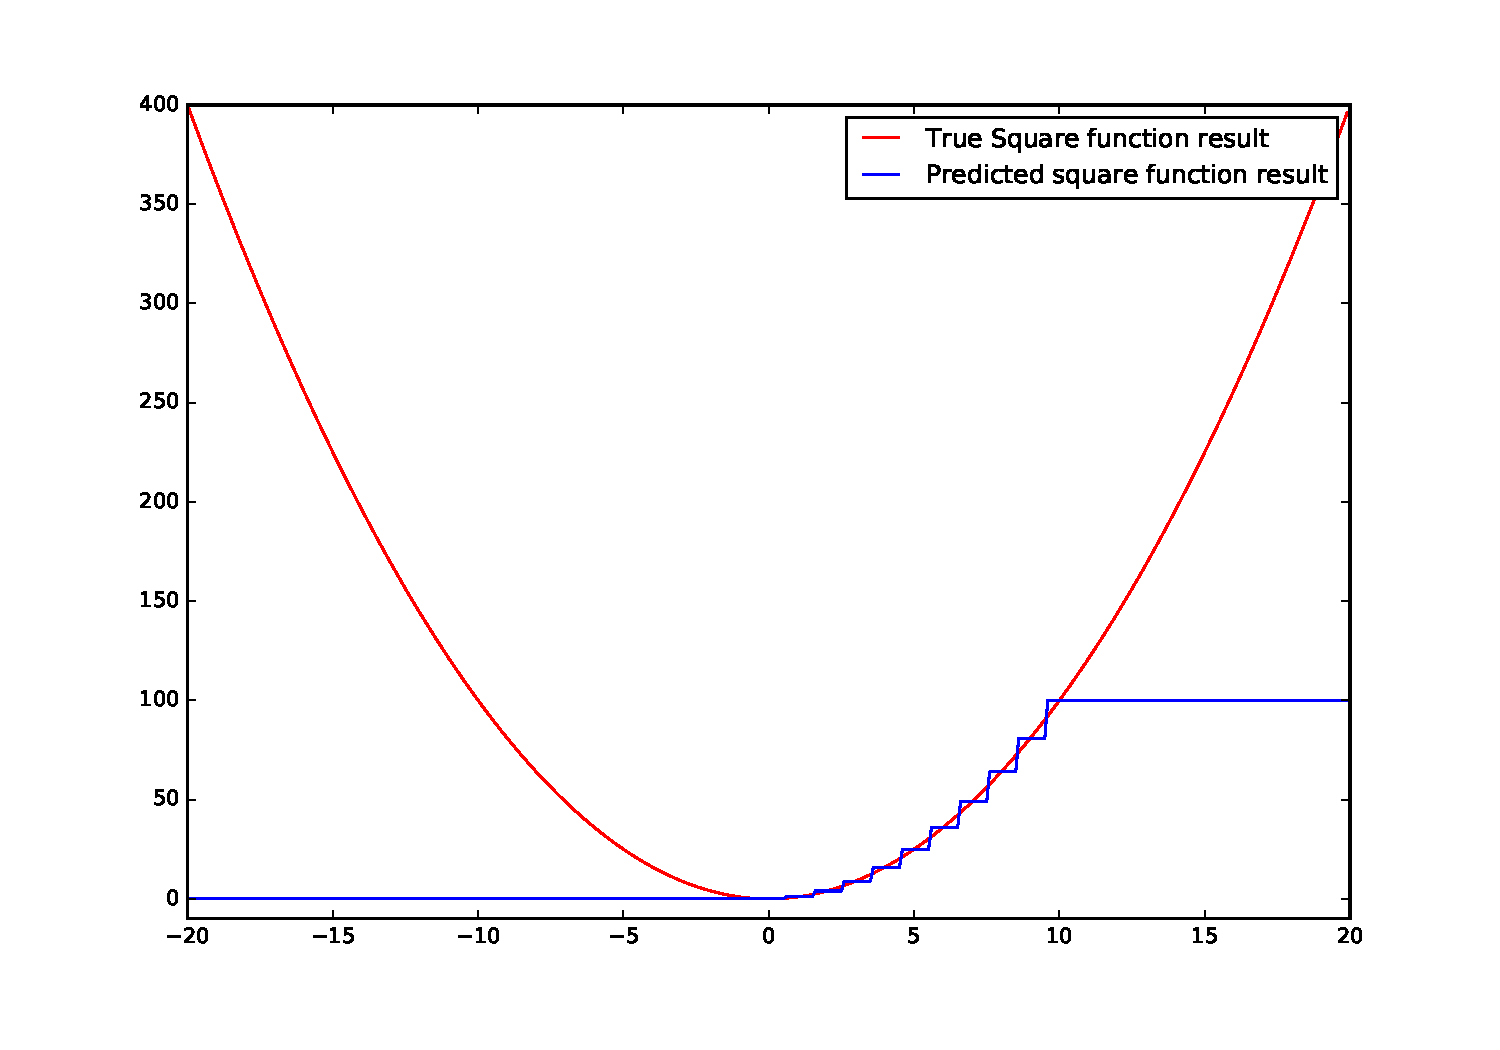
\includegraphics[width=\linewidth]{figures/clf_tree_plot.pdf}
        \caption{Classification Decision Test Results}
    \end{subfigure} %
    \begin{subfigure}{0.49\textwidth}
        \centering
        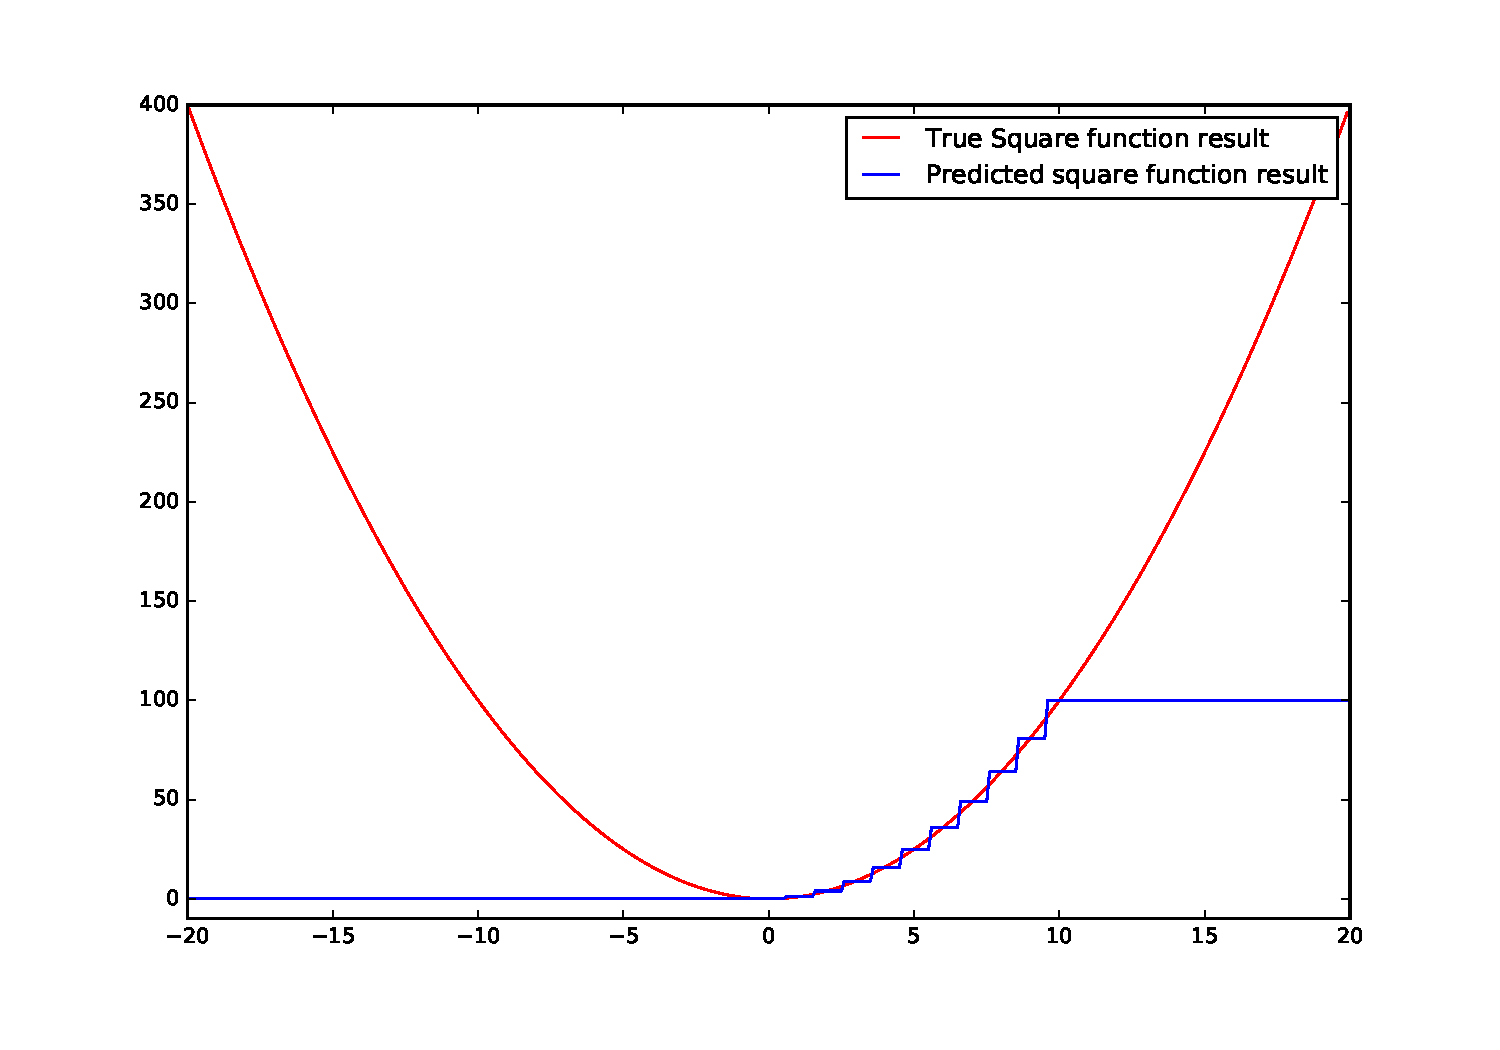
\includegraphics[width=\linewidth]{figures/reg_tree_plot.pdf}
        \caption{Regression Decision Test Results}
    \end{subfigure}
  \caption{Although a regression tree and a label classification tree have a different decision path with the same training data, they exhibit similar erronous behaviour when tested on input that ranges outside the training sample. The trees were trained on a dataset of simple square functions, where the inputs were numbers from 0 to 10 and output is the square of each number. Both decision trees show a jagged approximation of the square function between 0 and 10, which indicates some level of learning. However, the trees show very poor generalization outside the learning range. When tested on input that is below 0, the trees match to the closest label in the decision boundary, which is "0". A similar decision is made for input that is greater than 10, where the trees matches all numbers greater than 10 to the label of 10 ("100").}
  \label{fig:decision_tree_regression_and_classification}
\end{figure}

From this small experiment, the need for a different approach to supervised learning is obvious. Such a technique would need to generalize the mapping not to categorial labels and their limited space, but to an unlimited range of numbers. This method would solve a more conventional mathematical problem of function approximation. Another way to think about the problem is curve fitting: given input and output sets, the curve of the approximated function should pass---or be proximal---the points given in the sets. 
%The best fit for our function would be a curve that passes perfectly through all our data points.
As the aproximated curve moves further and futher away from the given points, the distance between the points and the curve increases, which we can use as a measurement of error (Fig. \ref{fig:error_lines}). The sum of this error can be expressed as

\begin{figure}[!h]
  \centering
  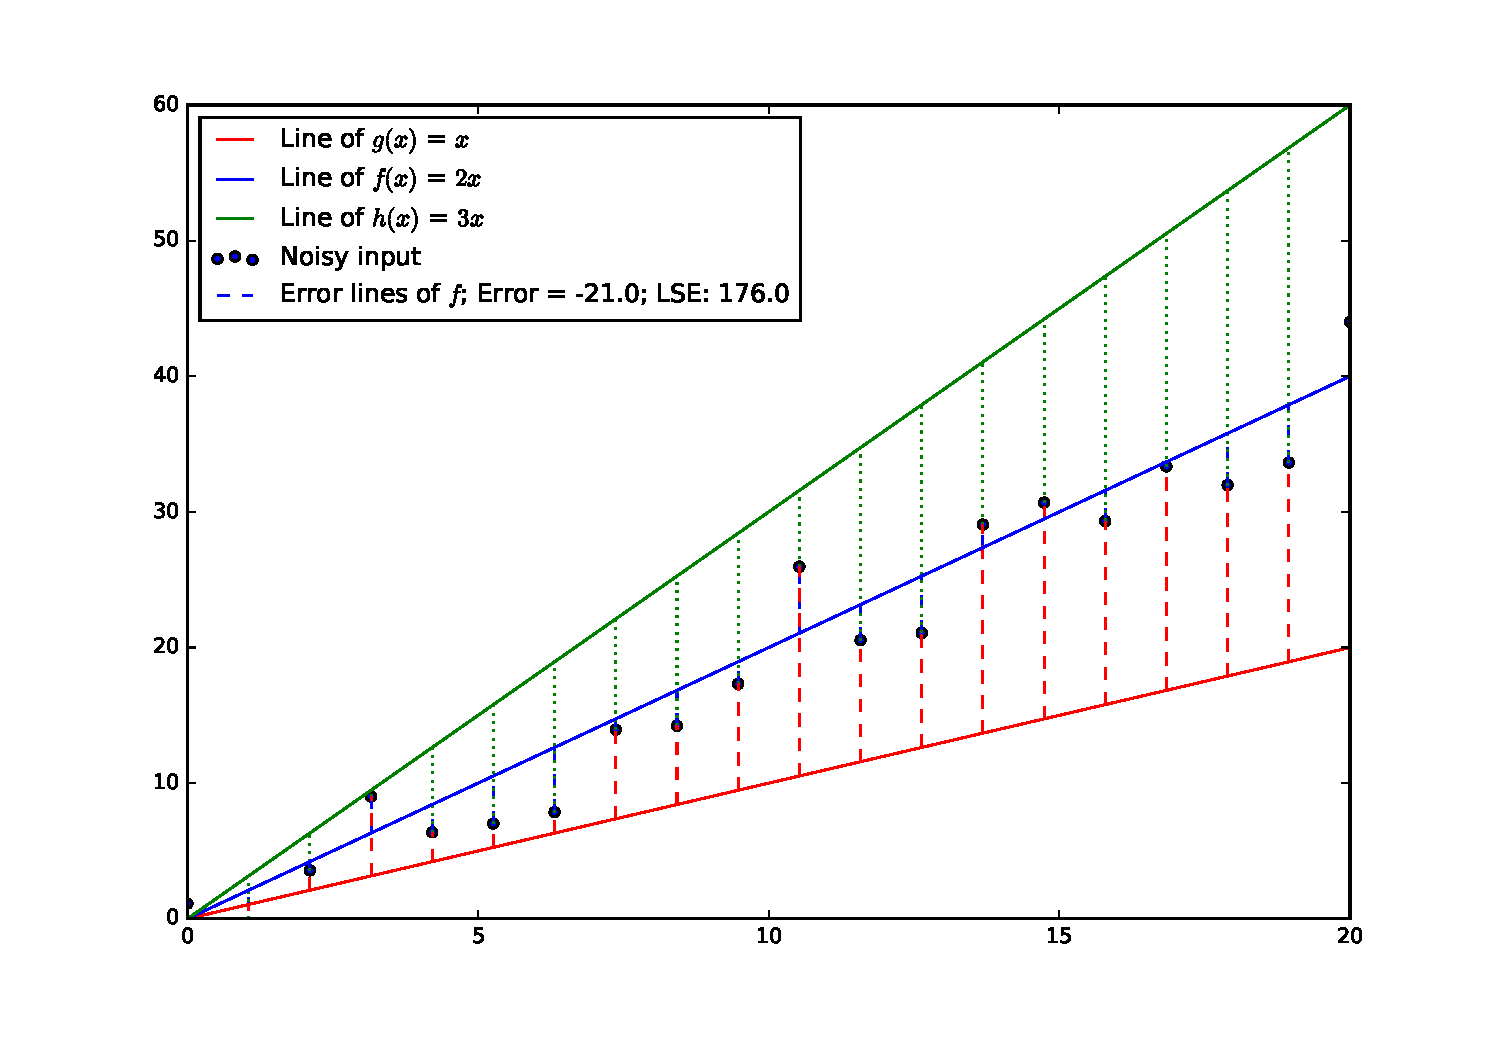
\includegraphics[width=\linewidth]{figures/error_lines.pdf}
  \caption{Different lines of fit and their errors (dashed and dotted lines) with respect to the noisy input data. Because $g(x)$ and $h(x)$ have larger error lines than $f(x)$, $f(x)$ is the best fit for the data out of the three drawn lines. Note that for $f(x)$, the negative and positive errors cancel out, leading to a sum of error of $-21$. This is allayed by suming the square of the erro instead, which results in a minimizable equation that evaluates to $176$.}
  \label{fig:error_lines}
\end{figure}

\begin{align*}
  Error &= \sum_{i=1}^n (y_i-f(x_i)),
\end{align*}

where for the $i$th data point $y_i$ represents the actual $y$ value and $f(x_i)$ represents the approximation of the regression line at $x_i$. Minimizing this error term ensures that our resulting function is the closes line fit to our data points. However, notice that in our error function, positive and negative errors will cancel out, leading to the assumption that "two wrongs make a right". To avoid this, we can either take the absolute value of the error, or the square. For mathematical convenience, the squared error is preferred. This results in the method of Least Squared Error (LSE) as given by

\begin{align}
\label{eq:least_square}
LSE &= \sum_{i=0}^n (y_i-f(x_i))^2  = \sum_{i=0}^n (y_i- b_0 - b_1x_i)^2
\end{align}

From this equation it can be shown that 

\begin{align}
b_1 &= \frac{\sum_{i=1}^n y_ix_i - \frac{\sum_{i=1}^n y_i \sum_{i=1}^n x_i}{n}}{\sum_{i=1}^n x_i^2 - \frac{\Big(\sum_{i=1}^n x_i \Big)^2}{n}}
\end{align}

and 
$$ b_0 = \bar y - b_1 \bar x $$

where $\bar y$ and $\bar x$ are the respective means of all $y$ and $x$ values \cite{Finney1996}. This formula guarantees a line of best fit that minimizes squared errors for linear data points. For cases when the data points do not display a linear behavior, they can be transformed into a space where they become more linear, linear regression applied, and the regression functions transformed back into the original space (Fig \ref{fig:log_regression}).

\begin{figure}[!h]
  \centering
    \begin{subfigure}{0.32\textwidth}
        \centering
        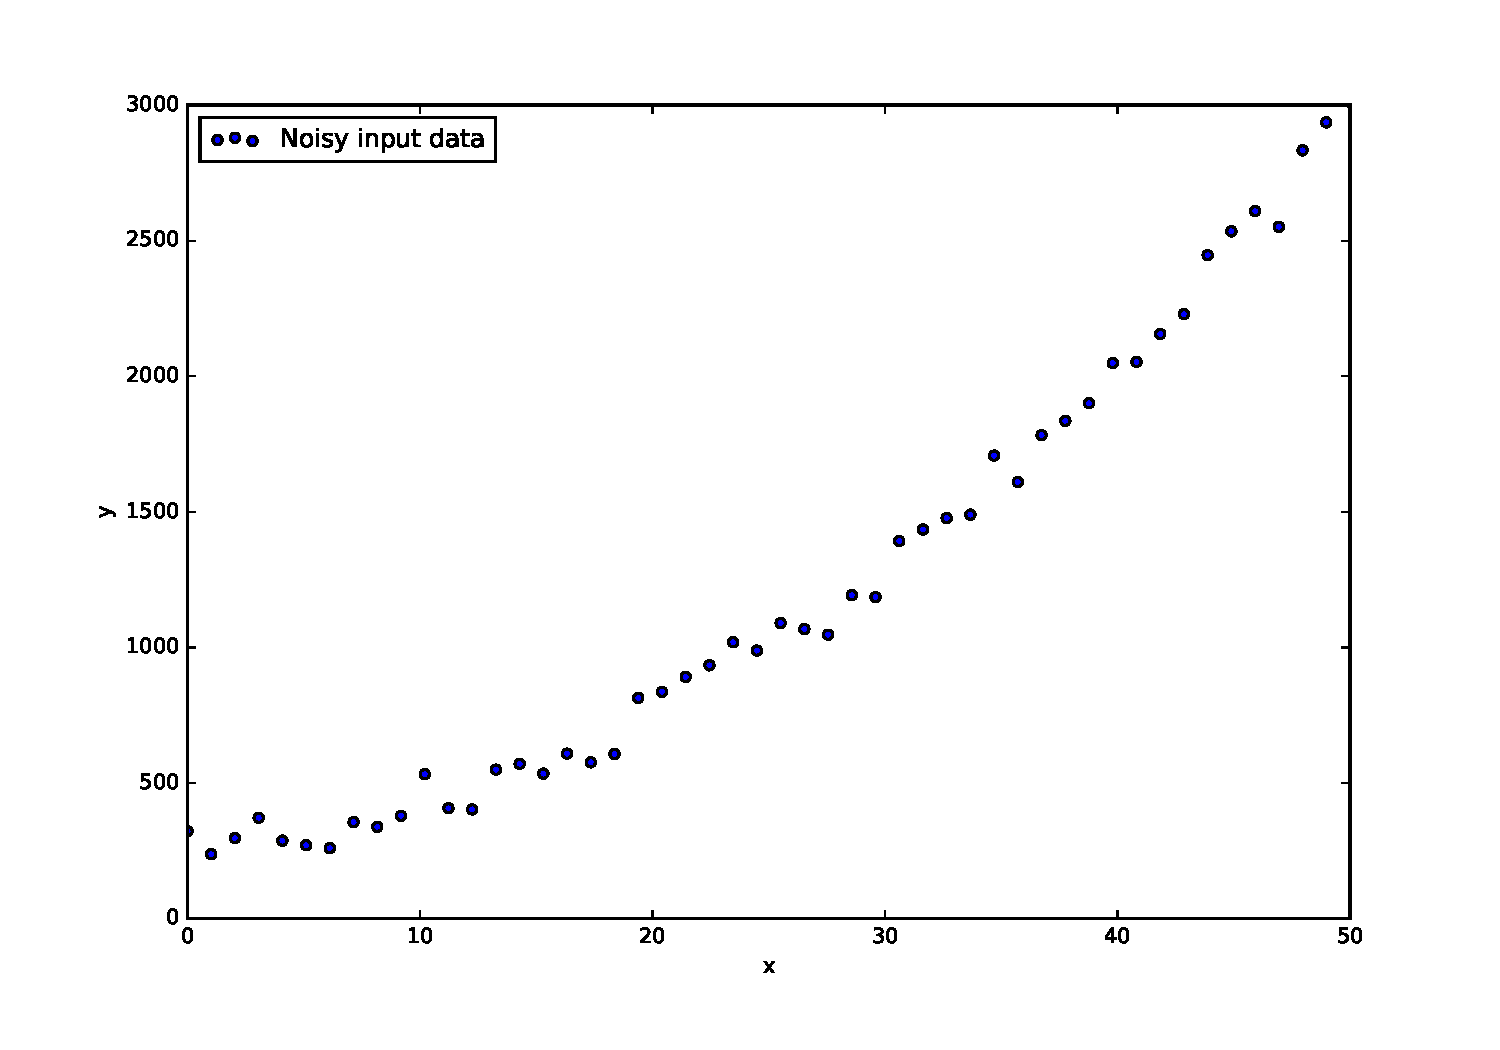
\includegraphics[width=\linewidth]{figures/regression_log_example_1.pdf}
    \end{subfigure}
  \begin{subfigure}{.32\textwidth}
        \centering
        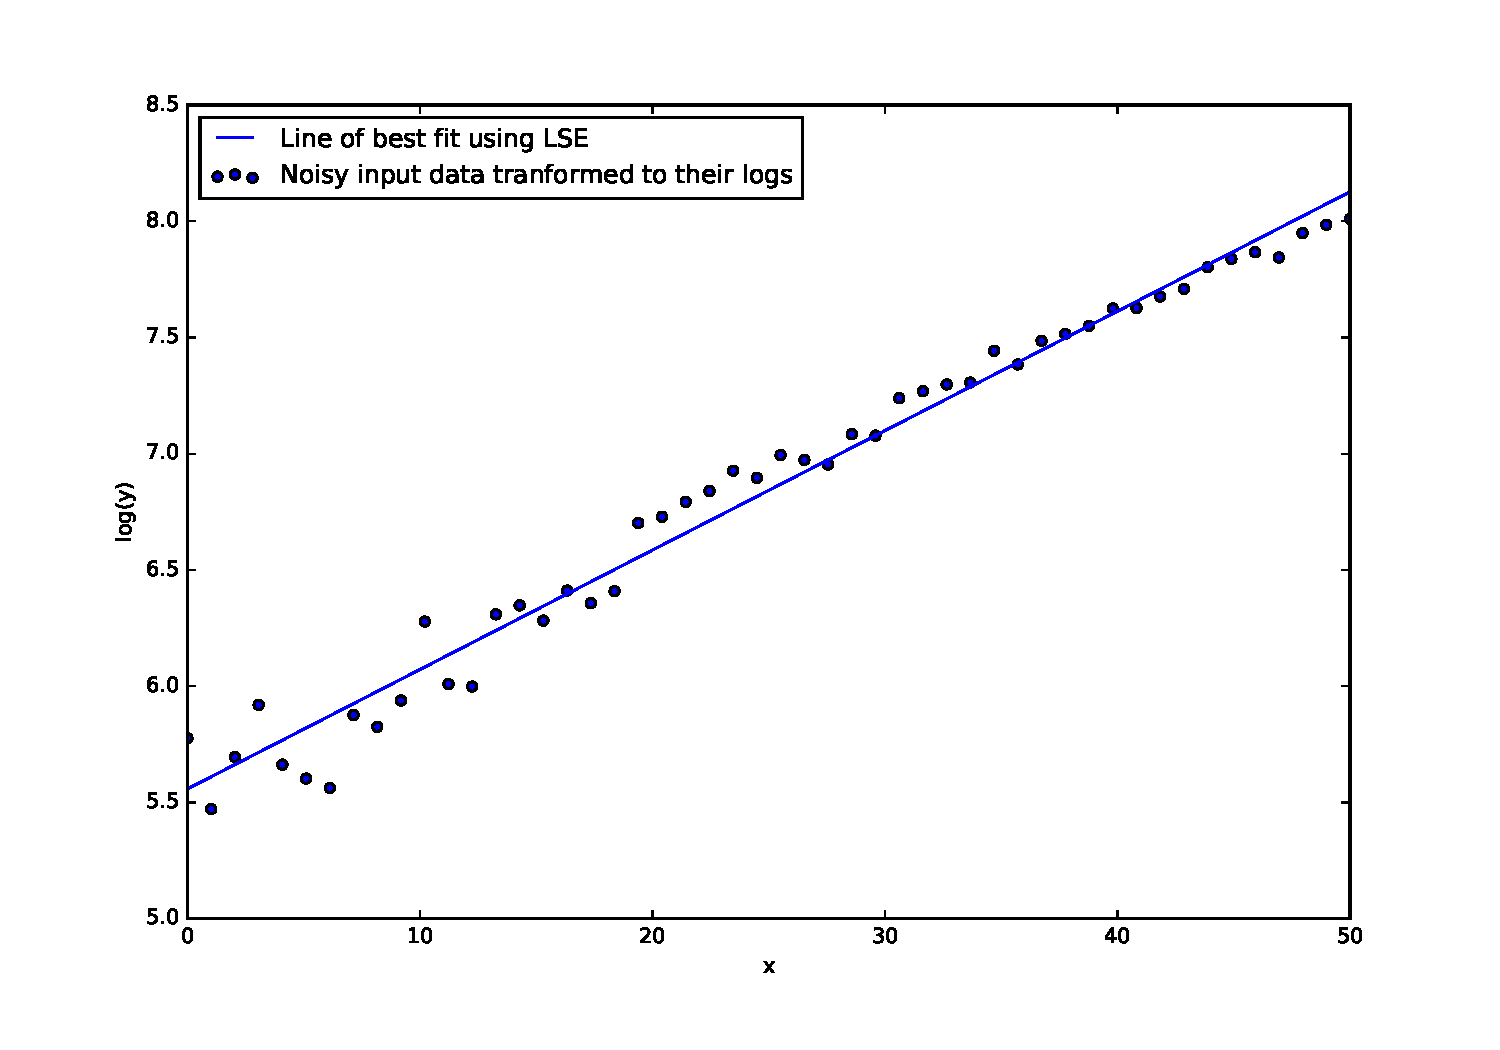
\includegraphics[width=\linewidth]{figures/regression_log_example_2.pdf}
    \end{subfigure}
    \begin{subfigure}{0.32\textwidth}
        \centering
        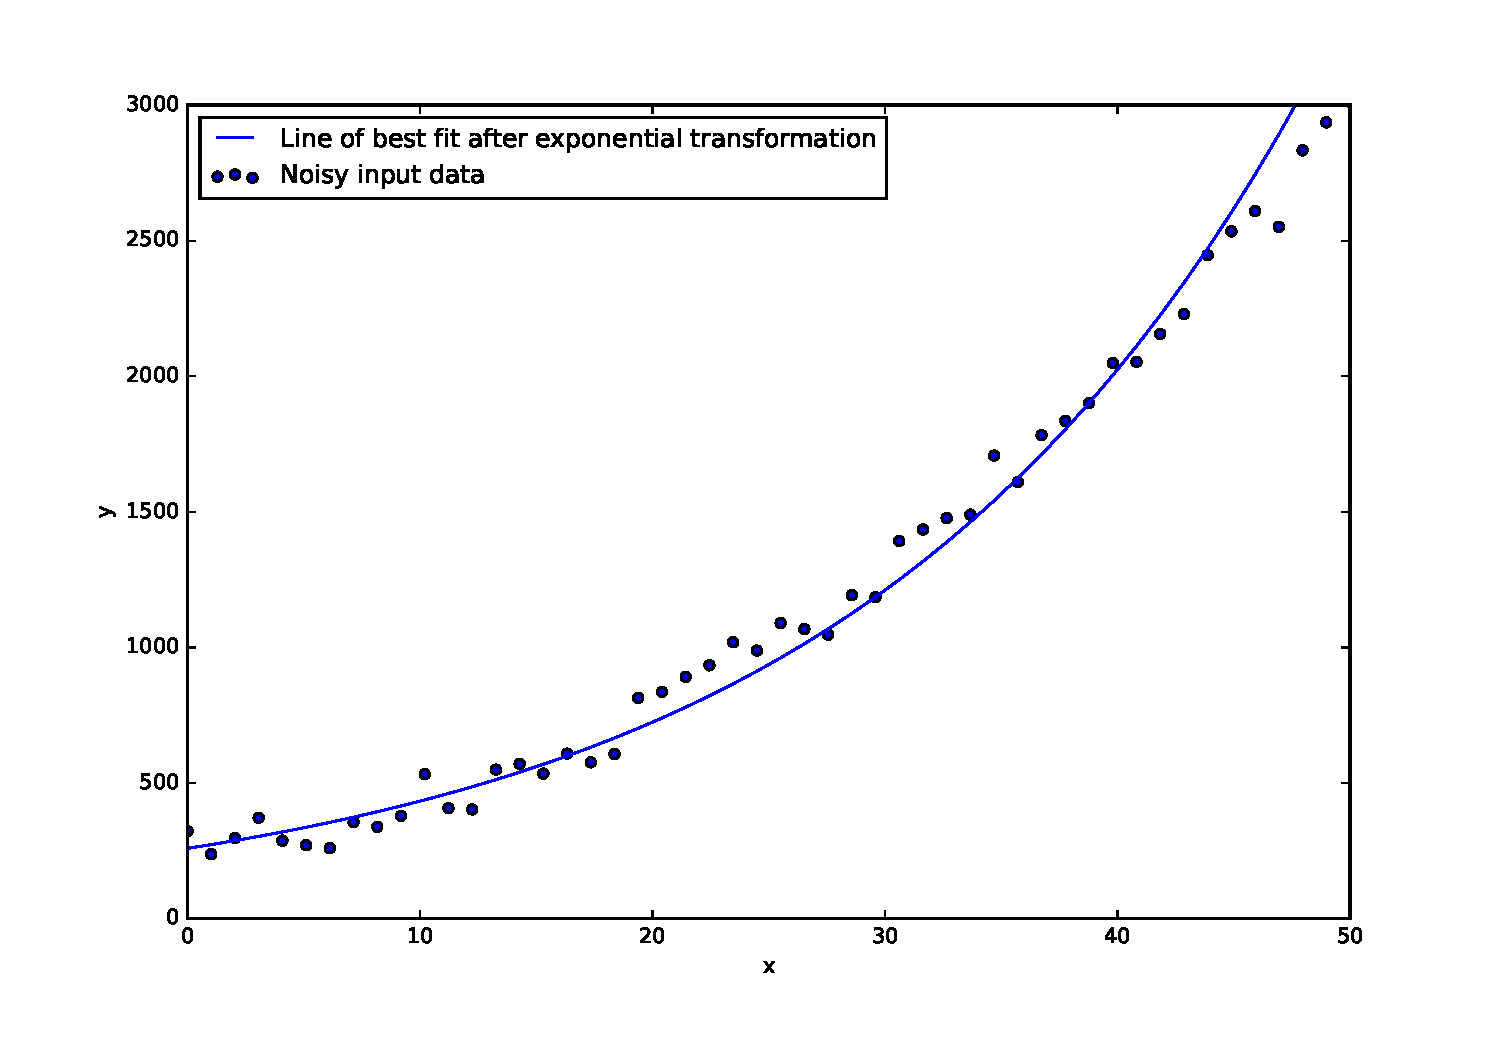
\includegraphics[width=\linewidth]{figures/regression_log_example_3.pdf}
    \end{subfigure}
  \caption{Finding line of least squared error for data with an exponential trend. First, the datapoints (Left) are transformed to their logs (Center). Then a line of best fit is found through linear regression (Center). The line is then transformed back to the original space by applying the exponential function (Right).}
  \label{fig:log_regression}
\end{figure}

TO BE CONTINUED WITH PERCEPTRON MODEL AND NEURAL NETWORKS

TO BE CONTINUED WITH SVM (SUPPORT VECTOR MACHINES)